\documentclass[conference]{IEEEtran}
\usepackage{graphicx}
\usepackage{booktabs}
\usepackage{url}

\begin{document}

\title{Phase 2 Split A: How Long Do People Wait?\\Linear Regression and MapReduce}
\author{\IEEEauthorblockN{Josh Hu}\IEEEauthorblockA{CTRL-Freaks, CSE 487 Fall 2026}}
\maketitle
\raggedbottom

\section{Overview}
Currently, we are looking for the number of days people wait for the completion of their 311 requests and if it is different between different districts of Buffalo. We had 528,079 requests \cite{data1}, \cite{data2} and 514,337 of them were closed. An open request does not have a closing date, so you cannot really calculate how many days were required to complete the request. Therefore, we decided to use closed requests.

For question 1, we selected linear regressions since they allowed us to make a fair comparison of districts through the same type of requests. The calculations performed using the MapReduce algorithm answer questions 1 and 3 based on the annual median wait of each district and the gaps between them from 2020 to 2026.

\section{Linear Regression}

\subsection{Why we chose it}
Essentially what we realized was that some districts just get more slow requests, like housing problems, so obviously it's going to be longer. It's not really the district's fault. Now the districts are compared on the same kinds of requests: pothole versus pothole, etc. Once we compared it like that, we found that in the North it's slightly slower.

\subsection{Training and tuning}
Our target was the resolution days. Categorical variables are council district, type, and opening month. As in Phase 1, 25 categories of type were used. One-hot encoding skips the first category of each variable. DELAWARE comes first alphabetically and, therefore, serves as a reference district. A special flag after switch denotes requests opened in the new system starting in May 2024. This allows for considering the difference between the system periods when estimating district coefficients. Altogether, we ended up with 44 features. Splitting the data in 80/20 with seed 42 via scikit-learn \cite{sklearn}, we trained on 411,469 records and tested on 102,868 records.

The target distribution is heavily tailed. While the median is about 4 days, there are requests which take more than 1,400 days to resolve. Thus, we trained two models. Version 1 is trained on resolution days as is, while Version 2 is trained on logarithm of days plus one. Predictions made by Version 2 are then converted to days. We compare two models against the baseline which makes predictions of the training set median for all test requests.

\subsection{Metrics}
Log model was chosen based on mean absolute error (MAE). The lowest MAE of the three models is 12.3 days, which is achieved by the log model (Table \ref{tab:lr}). The raw-days model has an MAE of 15.5 days and performs even worse than the median baseline on this criterion. The $R^2$ on the log-transformed target scale is 0.290: the model explains 29\% of variance in the target variable.

\begin{table}[h]
\centering
\caption{Test-set results for the baseline and two regression models}
\label{tab:lr}
\begin{tabular}{lcc}
\toprule
Model & $R^2$ (log) & MAE \\
\midrule
Baseline (median) & -0.012 & 13.56 \\
Raw days & -0.143 & 15.54 \\
Log days & 0.290 & 12.30 \\
\bottomrule
\end{tabular}
\end{table}

The log-scale $R^2$ of 0.29 shows the extent to which our model fails. Factors like crew availability, daily weather conditions, and request severity are missing from our dataset. Two requests may coincide on all recorded features yet take different times to be closed. We use the adjusted district coefficients to answer our comparison question, but the accuracy of our model leaves some room for improvement.

To analyze the impact of every feature group, we fit three more linear regressions, using log-transformed target. In each of them, only district, request type, or opening month was used. The $R^2$ for the type was 0.277, which is close to the full model. The $R^2$ values for district and month were 0.002 and 0.007 correspondingly. Type of the request was the most influential group among the three.

\subsection{What it tells us}
Figure \ref{fig:district} shows the district coefficients expressed in percentage form, with DELAWARE as the baseline. In this comparison, request type, opening month, and after switch are held constant. The percentages should be handled cautiously, since we estimated the log of resolution days + 1, so they refer to the back-transformation of the prediction + 1 day, not just the resolution days. Most differences are less than 5\%. The largest positive difference is NORTH, which is around 13.5\% higher than DELAWARE. The largest negative difference is SOUTH, which is around 5.8\% lower than DELAWARE.

\begin{figure}[h]
\centering
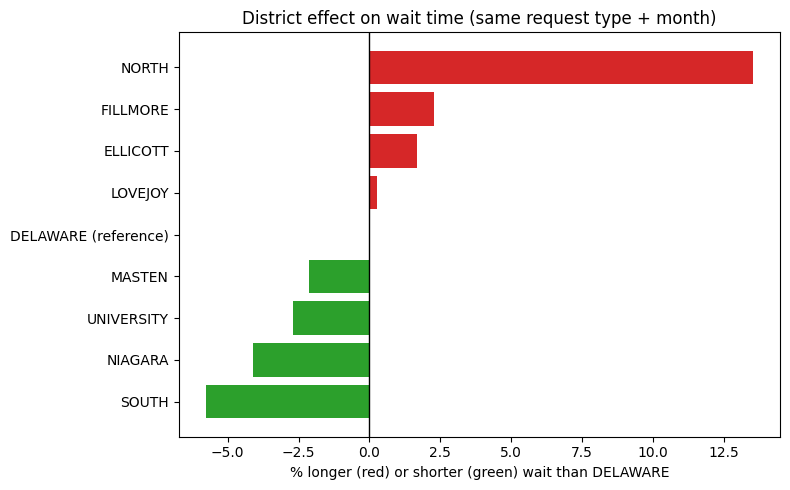
\includegraphics[width=\columnwidth]{figures/district_effect.png}
\caption{District differences from DELAWARE with other features held fixed, expressed as percentages of predicted days plus one.}
\label{fig:district}
\end{figure}

As an example of the adjustment effect, UNIVERSITY has the largest median in raw form, but its adjusted estimate is around 2.7\% lower than DELAWARE on the days + 1 scale. It may be that the difference in request types accounts for some of this. There could still be other differences between the districts. We compared predictions to observed resolution days for a sample of 5,000 test cases (Figure \ref{fig:scatter}). The predictions span a much smaller range than the observations, and do not capture the long wait times.

\begin{figure}[h]
\centering
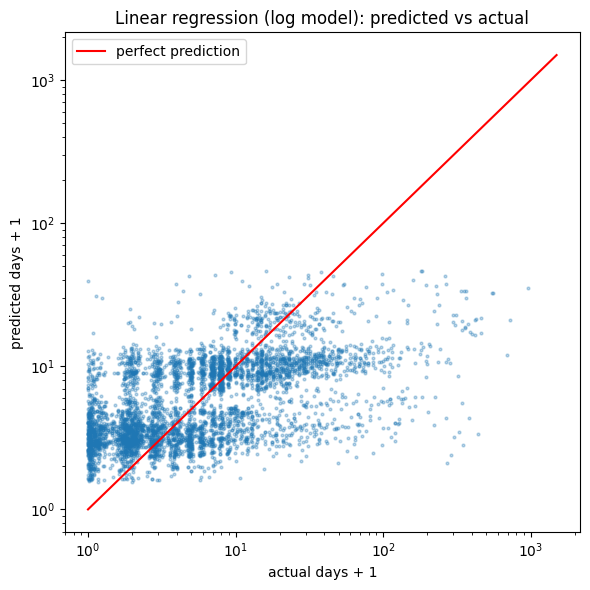
\includegraphics[width=0.85\columnwidth]{figures/predicted_vs_actual.png}
\caption{Actual and predicted resolution days for 5,000 test requests, shown on a log scale.}
\label{fig:scatter}
\end{figure}

\section{MapReduce}

\subsection{Why we chose it}
In the case of MapReduce, the problem consisted in computing 63 medians of districts and years out of 514,337 closed requests. It is possible to process rows independently using mappers, which output a key and wait time. The reducer computes the output for each key \cite{mapreduce}. Medians were selected since some outliers in wait times greater than 1,000 days could raise the average. In order to get the median of the group, our shuffle gathers all of its wait times and sends them to the reducer. Computing a median of medians of chunks will not, in general, yield the median of all requests.

\subsection{How we built it}
We wrote map, shuffle, and reduce in plain Python on one computer. Breaking up the input into 4 chunks of roughly 128,585 closed requests corresponds to how the work could be split to run on 4 computers. For each record, the mapper outputs the district and year pair with resolution days as the value. In the shuffle phase, we use a dictionary to store values that match with the key. The reducer sorts the list and computes the median. There are no parameters to be estimated here and no models to be trained. We provide a grouping and a statistic. For the comparison of the systems, we re-run the analysis using district and system period as the key with periods before and after May 2024.

\subsection{Metrics}
The medians of all the districts and years coincided with those computed using pandas groupby function. The overall computation time of MapReduce was 0.2 seconds. Consistency with pandas tests the implementation, but not the impact of excluding open requests. The years with an open rate from 0\% to 1.9\% were predominant; the open rates were 5.8\% and 8.4\% for 2024 and 2026 years correspondingly. If long wait times correlate with incompleteness of the requests, then the medians of closed requests will be underestimated. We thus have more reservations regarding the latest years.

\subsection{What it tells us}
The yearly medians in the districts are shown in Figure \ref{fig:lines}. In most districts, medians increased between 2020 and 2024, and the gaps between the districts were more pronounced after the change in the system. We measured the annual gaps as the difference between the maximum and minimum district median (Table \ref{tab:gap}, Figure \ref{fig:gap}). These gaps represent the observed waits and do not take the request type into account.

\begin{figure}[h]
\centering
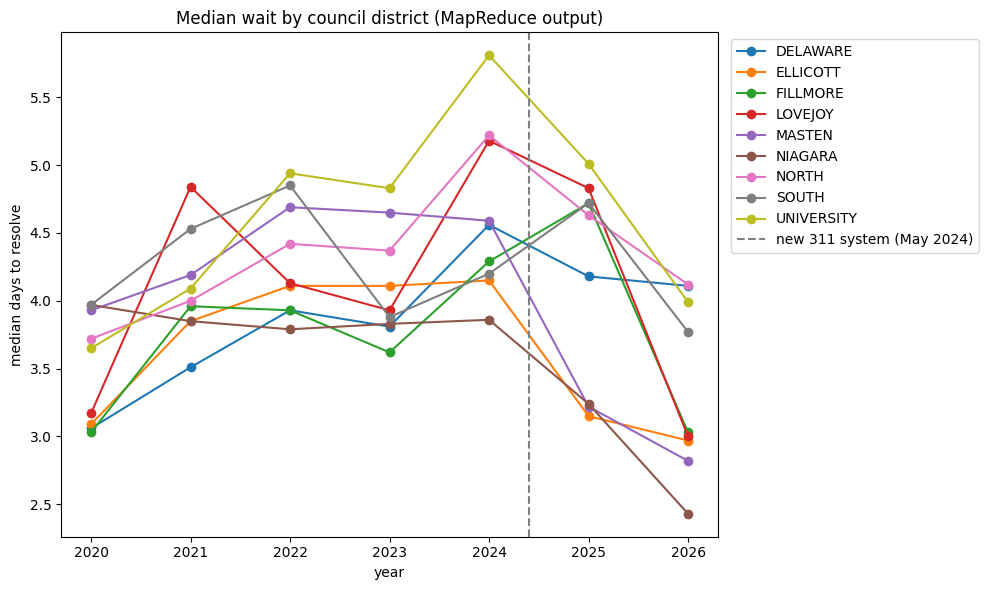
\includegraphics[width=\columnwidth]{figures/median_by_district.png}
\caption{Annual median resolution days for each council district. The system changed in May 2024, marked by the dashed line.}
\label{fig:lines}
\end{figure}

\begin{table}[h]
\centering
\caption{Districts with the highest and lowest annual median resolution days}
\label{tab:gap}
\begin{tabular}{lllc}
\toprule
Year & Slowest & Fastest & Gap \\
\midrule
2020 & NIAGARA (3.97) & FILLMORE (3.03) & 0.94 \\
2021 & LOVEJOY (4.84) & DELAWARE (3.51) & 1.33 \\
2022 & UNIVERSITY (4.94) & NIAGARA (3.79) & 1.15 \\
2023 & UNIVERSITY (4.83) & FILLMORE (3.62) & 1.21 \\
2024 & UNIVERSITY (5.81) & NIAGARA (3.86) & 1.95 \\
2025 & UNIVERSITY (5.01) & ELLICOTT (3.15) & 1.86 \\
2026 & NORTH (4.12) & NIAGARA (2.43) & 1.69 \\
\bottomrule
\end{tabular}
\end{table}

\begin{figure}[h]
\centering
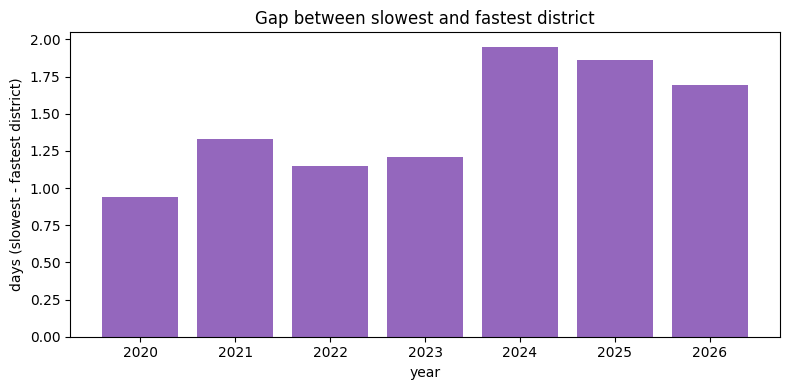
\includegraphics[width=\columnwidth]{figures/district_gap.png}
\caption{Annual difference between the highest and lowest district median wait.}
\label{fig:gap}
\end{figure}

In 2020, the gap was 0.94 days. It grew to 1.95 days in 2024 and decreased to 1.69 days in 2026. In the comparison of the system periods, the gap is 0.71 days before May 2024 and 1.92 days thereafter. Not all districts had an increase in medians: NIAGARA and MASTEN had smaller medians during the new-system period, while DELAWARE, NORTH, and LOVEJOY medians were about a day higher. Regarding research question Q3, we observe a larger district gap in the latter part of our observation period than in its beginning. This growth cannot be attributed to the system change since closure times could have been coded differently in the two systems, and the recent years included requests that have not yet been closed.

\section{Limitations}
However, there are limits to both of these. In the first phase, missing council districts were assigned for 2020 and 2021 based on the district boundaries from 2011. They coincide with the current boundaries about 90 percent of the time, which means some requests could have been assigned differently based on the current boundaries. The regression model accounts for only about 29\% of the variance and has no data on the availability of crews and severity of requests.

\begin{thebibliography}{1}
\bibitem{data1} City of Buffalo, ``311 Service Requests (July 2008 - May 2024),'' Buffalo Open Data. \url{https://data.buffalony.gov/Quality-of-Life/311-Service-Requests-July-2008-May-2024-/whkc-e5vr}
\bibitem{data2} City of Buffalo, ``311 Service Requests (May 2024 - Present),'' Buffalo Open Data. \url{https://data.buffalony.gov/Quality-of-Life/311-Service-Requests-May-2024-Present-/3tj7-3tdz}
\bibitem{mapreduce} J. Dean and S. Ghemawat, ``MapReduce: Simplified Data Processing on Large Clusters,'' in \emph{Proc. OSDI}, 2004.
\bibitem{sklearn} F. Pedregosa et al., ``Scikit-learn: Machine Learning in Python,'' \emph{JMLR}, vol. 12, pp. 2825-2830, 2011.
\bibitem{vanderplas} J. VanderPlas, \emph{Python Data Science Handbook}. O'Reilly, 2016.
\end{thebibliography}

\end{document}
